\subsection{Ejecución de prueba Kruskal-Wallis para comparar las diferencias entre la dopamina segregada antes y después de tocar Piano, Cello y Flauta}
A continuación se encuentran las diferencias entre la medición de dopamina de personas seleccionadas aleatoriamente antes de tocar un instrumento y después de tocar un instrumento, la resta de las mediciones antes de tocar instrumentos y después produjeron la siguiente tabla.

Es importante considerar lo siguiente: 
\begin{itemize}
    \item Cuando los datos son negativos significa que el nivel de dopamina después de tocar un instrumento disminuyó en comparación al nivel de dopamina antes de tocar un instrumento.
    \item Cuando los datos son 0 significa que el nivel de dopamina se mantuvo constante durante el experimento. 
    \item Cuando los datos son positivos significa que al tocar dicho instrumento la dopamina aumentó en comparación al nivel de dopamina segregada antes de tocar el instrumento.
\end{itemize}

Queremos investigar si el nivel de dopamina segregado después de tocar alguno de los instrumentos en cuestión (piano, cello o flauta) es diferente según cuál instrumento se esté tocando.

\begin{center}
    \begin{tabular}{ |ccc| }
        \hline  
            PIANO & CELLO & FLAUTA \\ 
        \hline
            0.5 & 0.3 & 0.6  \\
            0.1 & 0.4 & 0.1   \\
            -0.1 & 0.5 & 0.1   \\
            -0.3 & 0.3 & 0   \\
            -0.4 & 0.3 & -0.9   \\
            1.2 & -0.1 & -0.5   \\
            -0.4 & 0.2 & 0.3   \\
            -0.2 & 0.4 & 0.7   \\
            -0.7 & 0.2 & 0.6   \\
            0 & 0.4 & 0  \\
            -0.6 & 0.9 & 0.3   \\
            -0.5 & 0 & -0.1  \\ 
        \hline
    \end{tabular}
\end{center}

Por la naturaleza del experimento procederemos a aplicar la prueba Kruskal-Wallis para comparar las tres poblaciones.

\begin{enumerate}
    \item Justificación de la prueba: 
        \begin{itemize}
            \item $n_{1,2,3} \geq 5$
            \item Puesto al hecho que tenemos que comparar varias poblaciones procedemos a usar esta prueba. 
        \end{itemize}
    \item Estadístico de prueba: poblaciones.
    \item Hipótesis: 
        \begin{enumerate}
            \item $H_0$: todas las poblaciones son iguales. %$\text{población}_1 = \text{población}_2 = \text{población}_3$.
            \item $H_a$: no todas las poblaciones son iguales. %$\text{población}_1 \neq \text{población}_2 \neq \text{población}_3$.
        \end{enumerate}
    
    \item Significancia: $\alpha = 0.05$
    \item Estadístico de prueba: 
        \begin{itemize}
            \item Establecemos las variables preliminares:  
                \begin{itemize}
                    \item $k=3$ (3 muestras).
                    \item $n_P = 12, \qq n_C = 12, \qq n_F = 12$ ($n_P$ númbero de observaciones de piano, $n_C$ número de observaciones de cello, $n_F$ número de observaciones de flauta).
                    \item $n_T = 36$ (número total de observaciones).
                    \item $R_P = 149.5, \qq R_C = 288, \qq R_F = 288.5 $ ($R_P$ suma de rangos de piano, $R_C$ suma de rangos de cello, $R_F$ suma de rangos de flauta).
                        \begin{center}
                            \begin{tabular}{|lll|}
                                \hline
                                PIANO & CELLO & FLAUTA \\
                                \hline
                                30.5 & 24 & 32.5 \\
                                18 & 28 & 18 \\
                                11 & 30.5 & 18 \\
                                8 & 24 & 14.5 \\
                                6.5 & 24 & 1 \\
                                36 & 11 & 4.5 \\
                                6.5 & 20.5 & 24 \\
                                9 & 28 & 34 \\
                                2 & 20.5 & 32.5 \\
                                14.5 & 28 & 14.5 \\
                                3 & 35 & 24 \\
                                4.5 & 14.5 & 11 \\
                                \textbf{149.5} & \textbf{288} & \textbf{228.5} \\
                                \hline
                            \end{tabular}
                        \end{center}
                    
                    \item $gl=2$ (grados de libertad para $\chi^2$). 
                    \item $\displaystyle \sum_{i=1}^{k}\frac{R^2_i}{n_i} = 13125.54167$
                        \[
                            \sum_{i=1}^{3} \frac{R^2_i}{n_i} = \p{\frac{149.5^2}{12}}  + \p{\frac{288^2}{12}}  + \p{\frac{288.5^2}{12}}  =  13125.54167 \\ 
                        \]
                \end{itemize}
            
            \item Procedemos a calcular el estadístico $H = 7.248123123$. 
                \begin{center}
                   \begin{align*}
                       H &= \sqb{\frac{12}{n_T(n_T+1)}\sum_{i=1}^{k}\frac{R^2_i}{n_i}} -3(n_T+1) \\ 
                       &= \sqb{\frac{12}{36 \times (36 + 1)}\times 13125.54167} -3\times(36 + 1) \\ 
                       &= \sqb{0.009009009 \times 13125.54167} -111 \\ 
                       &= 7.248123123 \\ 
                   \end{align*}
                \end{center}
            
            \item Procedemos a sacar el $valor-p = 0.026674118$:
                \begin{figure}[H]
                    \centering
                    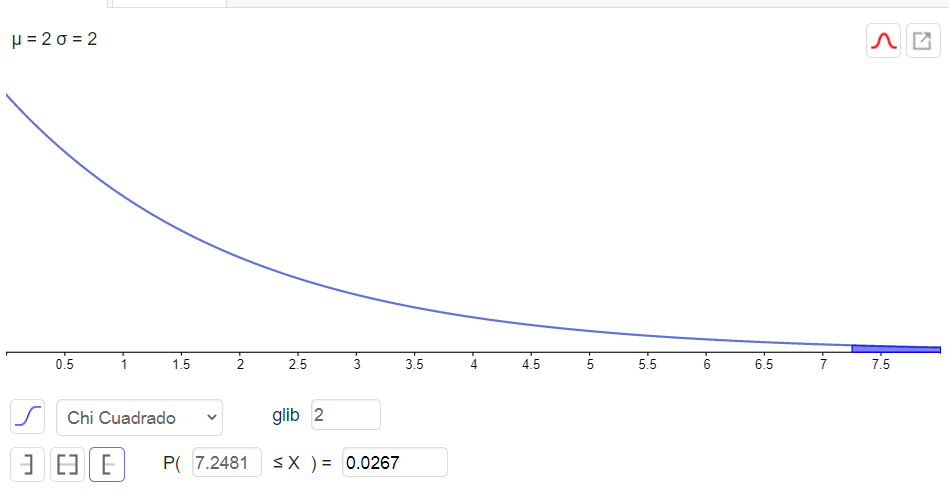
\includegraphics[width=0.8\textwidth]{./appendages/valor-pKW.png}
                    \caption{Geogebra: sacado de la calculadora de probabilidad $\chi^2$ de Geogebra}
                \end{figure}
                \begin{itemize}
                    \item $valor-p= 0.026674118$
                \end{itemize}
        \end{itemize}
        
        \begin{itemize}
            \item Criterio de rechazo: rechazar $H_0$ si $valor-p \leq \alpha$.
                \begin{itemize}
                    \item $valor-p = 0.026674118$
                    \item $\alpha = 0.05$
                    \item $0.026674118 \leq 0.05$. Verdadero. Rechazar $H_0$. 
                \end{itemize}
        \end{itemize}

    \item Conclusión: Con una significancia de 0.05 se puede afirmar que no todas las poblaciones son iguales y si hay diferencia estadísticamente significativa en los aumentos de dopamina, de acuerdo al instrumento que se toca.
\end{enumerate}

Para dar refuerzo estadístico a la prueba anterior, conduciremos dos pruebas Mann-Whitney-Wilcoxon para ver cuál población difiere de cuál y encontrar posibles casos en los que encontraremos que dos muestras producen una distribución de muestreo idéntica y otras en las que no.

%----------------------------------------------------------------------------------------

\subsection{Ejecución de prueba Mann-Whitney-Wilcoxon para comparar si hay diferencia estadística entre la población del Piano y Cello}

Dada la siguiente información: los datos se producen a partir de la diferencia entre el nivel de dopamina previo a tocar un instrumento y el nivel de dopamina después de tocarlo.
\begin{center}
    \begin{tabular}{ |cc| }
        \hline
        PIANO & CELLO \\
        \hline
        0.5 & 0.3 \\
        0.1 & 0.4 \\
        -0.1 & 0.5 \\
        -0.3 & 0.3 \\
        -0.4 & 0.3 \\
        1.2 & -0.1 \\
        -0.4 & 0.2 \\
        -0.2 & 0.4 \\
        -0.7 & 0.2 \\
        0 & 0.4 \\
        -0.6 & 0.9 \\
        -0.5 & 0 \\
        \hline
    \end{tabular}
\end{center}

\begin{enumerate}
    \item Justificación de la prueba:
        \begin{itemize}
            \item Se eligió esta prueba al considerar lo siguiente: 
            \item $n \geq 7$ 
            \item Poblaciones independientes.
            \item No es una muestra pareada.
            \item Procedemos a aplicar Mann-Whitney-Wilcoxon.
        \end{itemize}
    \item Parámetro de interés: poblaciones.
    \item Hipótesis: 
        \begin{enumerate}
            \item $H_0$: las poblaciones son iguales.
            \item $H_a$: las poblaciones son diferentes.
        \end{enumerate}
    
    \item Significancia: $\alpha = 0.05$ 
    \item Estadístico de prueba: 
        \begin{itemize}
            \item Establecer variables preliminares: 
                \begin{itemize}
                    \item $n_P = 12, \qq  n_C = 12$ ($n_P$ número de observaciones de piano, $n_C$ número de observaciones de cello).
                    \item $R_P = 104.5, \qq R_C = 195.5$ ($R_P$ suma de rangos de piano, $R_C$ suma de rangos de cello).
                        \begin{center}
                            \begin{tabular}{ |cc| }
                                \hline
                                PIANO & CELLO \\ 
                                \hline
                                21.5 & 16 \\
                                12 & 19 \\
                                8.5 & 21.5 \\
                                6 & 16 \\
                                4.5 & 16 \\
                                24 & 8.5 \\
                                4.5 & 13.5 \\
                                7 & 19 \\
                                1 & 13.5 \\
                                10.5 & 19 \\
                                2 & 23 \\
                                3 & 10.5 \\
                                \textbf{104.5} & \textbf{195.5} \\ 
                                \hline
                            \end{tabular}
                        \end{center}
                    \item $W = 104.5 + 0.5 = 105$ ($W$ más 0.5 puesto al factor de corrección de continuidad).
                \end{itemize}
            
            \item Procedemos a calcular $\mu_W = 150$.
                \begin{center}
                   \begin{align*}
                       \mu_W &= \frac{n_1(n_1+n_2+1)}{2}\\
                       &= \frac{12\times(12 + 12 + 1)}{2} \\ 
                       &= \frac{12\times 25}{2} \\ 
                       &= \frac{300}{2} \\ 
                       &= 150 \\  
                   \end{align*}
                \end{center}

            \item Procedemos a calcular $\sigma_W = 17.32050808$
                \begin{center}
                   \begin{align*}
                       \sigma_W &= \sqrt{\frac{n_1\times n_2(n_1+n_2+1)}{12}} \\
                       &= \sqrt{\frac{(12)\times(12)\times(12+12+1)}{12}} \\
                       &= \sqrt{\frac{3,600}{12}} \\
                       &= \sqrt{300} \\
                       &= 17.32050808 \\
                   \end{align*}
                \end{center}
            
            \item Procedemos a calcular $z = -2.598076211$
                \begin{center}
                   \begin{align*}
                       z &= \frac{(W+0.5)-\mu_W}{\sigma_W} \\
                       &= \frac{(104.5+0.5)-150}{17.32050808} \\
                       &= \frac{105-150}{17.32050808} \\ 
                       &= -\frac{45}{17.32050808} \\
                       &= -2.598076211 \\ 
                   \end{align*}
                \end{center}
            
            \item Procedemos a calcular el $valor-p = 0.00937$
                \begin{itemize}
                    \item Utilizando la función de Excel \verb|=2*NORM.S.DIST(-2.598076211,1)|= 0.00937, obtenemos el $valor-p$.
                \end{itemize}
        \end{itemize}
        \begin{itemize}
            \item Criterio de rechazo: rechazar $H_0$ si $valor-p\leq \alpha$. 
                \begin{itemize}
                    \item $valor-p = 0.009374768$
                    \item $\alpha = 0.05$
                    \item $0.009374768 \leq 0.05$. Verdadero. Rechazar $H_0$.
                \end{itemize}
        \end{itemize}
    
    \item Conclusión: con significancia de 0.05 podemos afirmar que las muestras no provienen de la misma población y si hay diferencia estadísticamente significativa entre la dopamina segregada al después de tocar piano en comparación a la segregada después a tocar cello. 
\end{enumerate}


%----------------------------------------------------------------------------------------

\subsection{Ejecución de prueba Mann-Whitney-Wilcoxon para comparar si hay diferencia estadística entre la población del Cello y Flauta}

Dada la siguiente información: los datos se producen a partir de la diferencia entre el nivel de dopamina previo a tocar un instrumento y el nivel de dopamina después de tocarlo.
\begin{center}
    \begin{tabular}{ |cc| }
        \hline
        CELLO & FLAUTA \\
        \hline
        0.3 & 0.6 \\
        0.4 & 0.1 \\
        0.5 & 0.1 \\
        0.3 & 0 \\
        0.3 & -0.9 \\
        -0.1 & -0.5 \\
        0.2 & 0.3 \\
        0.4 & 0.7 \\
        0.2 & 0.6 \\
        0.4 & 0 \\
        0.9 & 0.3 \\
        0 & -0.1 \\
        \hline
    \end{tabular}
\end{center}

\begin{enumerate}
    \item Justificación de la prueba:
        \begin{itemize}
            \item Se eligió esta prueba al considerar lo siguiente: 
            \item $n \geq 7$ 
            \item Poblaciones independientes.
            \item No es una muestra pareada.
            \item Procedemos a aplicar Mann-Whitney-Wilcoxon.
        \end{itemize}
    \item Parámetro de interés: poblaciones.
    \item Hipótesis: 
        \begin{enumerate}
            \item $H_0$: las poblaciones son iguales.
            \item $H_a$: las poblaciones son diferentes.
        \end{enumerate}
    
    \item Significancia: $\alpha = 0.05$ 
    \item Estadístico de prueba: 
        \begin{itemize}
            \item Establecer variables preliminares:
                \begin{itemize}
                    \item $n_C = 12, \qq  n_F = 12$ ($n_P$ número de observaciones de cello, $n_C$ número de observaciones de flauta).
                    \item $R_C = 170.5, \qq  R_F = 129.5$ ($R_C$ suma de rangos de cello, $R_F$ suma de rangos de flauta).
                    \item $W = 170 - 0.5$ ($W$ menos 0.5 por el factor de corrección de continuidad).
                \end{itemize}
            
            \item Procedemos a calcular $\mu_W = 150$.
                \begin{center}
                   \begin{align*}
                       \mu_W &= \frac{n_1(n_1+n_2+1)}{2}\\
                       &= \frac{12\times(12 + 12 + 1)}{2} \\ 
                       &= \frac{12\times 25}{2} \\ 
                       &= \frac{300}{2} \\ 
                       &= 150 \\  
                   \end{align*}
                \end{center}

            \item Procedemos a calcular $\sigma_W = 17.32050808$
                \begin{center}
                   \begin{align*}
                       \sigma_W &= \sqrt{\frac{n_1\times n_2(n_1+n_2+1)}{12}} \\
                       &= \sqrt{\frac{(12)\times(12)\times(12+12+1)}{12}} \\
                       &= \sqrt{\frac{3,600}{12}} \\
                       &= \sqrt{300} \\
                       &= 17.32050808 \\
                   \end{align*}
                \end{center}
            
            \item Procedemos a calcular $z = 1.154700538$
                \begin{center}
                   \begin{align*}
                       z &= \frac{(W-0.5)-\mu_W}{\sigma_W} \\
                       &= \frac{(170.5-0.5)-150}{17.32050808} \\
                       &= \frac{170-150}{17.32050808} \\ 
                       &= \frac{20}{17.32050808} \\
                       &= 1.154700538 \\ 
                   \end{align*}
                \end{center}
            
            \item Procedemos a calcular el $valor-p = 0.248213079$
                \begin{itemize}
                    \item Utilizando la función de Excel \verb|=2*(1-NORM.S.DIST(1.154700538,1))|= 0.248213079, obtenemos el $valor-p$.
                \end{itemize}
            
            \item Criterio de rechazo: rechazar $H_0$ si $valor-p\leq \alpha $: 
                \begin{itemize}
                    \item $valor-p=0.248213079$
                    \item $\alpha=0.05$ 
                    \item $0.248213079\leq 0.05$. Falso. No rechazar $H_0$. 
                \end{itemize}
        \end{itemize}
    
    \item Conclusión: Con significancia de 0.05 no hay suficiente evidencia afirmar que las muestras vienen de diferente población, puesto a que no se puede rechazar la $H_0$ no se puede afirmar que haya diferencia estadística entre la dopamina segregada al tocar el cello versus la dopamina segregada al tocar la flauta.
\end{enumerate}
